\documentclass{beamer}
\usetheme{CambridgeUS}

% Title page details:
\title{GoTalk}
\author{Swasti \and Shreya \and Krishika \and Samriddhi}
\date{\today}

\begin{document}

\begin{frame}
    \titlepage
    \centering HACKTIVISTS
\end{frame}

\begin{frame}{PROJECT AIM}
    To develop a real-time chat web application with chat history retrieval using Go, WebSocket and Firebase majorly.   
    \\
    Our main aim is to Learn the Go language and Firebase and learn how to establish a client-server connection using WebSocket .
\end{frame}

\section{Tech Stack}
\begin{frame}{Tech Stack}
    \begin{itemize}
        \item \textbf{Frontend}
        \begin{itemize}
            \item HTML/CSS
            \item JavaScript
            \item Bootstrap/Tailwind CSS
        \end{itemize}
        \item \textbf{Backend}
        \begin{itemize}
            \item Go (Golang)
            \item Gorilla WebSocket
            \item Firebase Realtime Database
        \end{itemize}
    \end{itemize}
\end{frame}

\section{Tasks Completed Till Now}

\begin{frame}{Tasks Completed Till Now}
    \begin{itemize}
        \item \textbf{Initial Setup:}
        \begin{itemize}
            \item Set up Go development environment.
            \item Created basic Go app with WebSocket support.
        \end{itemize}
        \item \textbf{Firebase Integration:}
        \begin{itemize}
            \item Set up Firebase Realtime Database for chat data storage.
        \end{itemize}
    \end{itemize}
\end{frame}

\begin{frame}{Tasks Completed Till Now (Contd.)}
    \begin{itemize}
        \item \textbf{Bidirectional Communication:}
        \begin{itemize}
            \item Implemented WebSocket-based communication.
            \item Established real-time messaging.
        \end{itemize}
        \item \textbf{Past Chat Retrieval:}
        \begin{itemize}
            \item Retrieved past chats from Firebase.
            \item Displaying past chats.
        \end{itemize}
    \end{itemize}
\end{frame}

\begin{frame}{Tasks Completed Till Now (Contd.)}
    \begin{itemize}
        \item \textbf{Basic UI Development:}
        \begin{itemize}
            \item Added basic styles for chat interface.
            \item Created simple layout for message display.
        \end{itemize}
    \end{itemize}
\end{frame}

\section{New Tasks Done}

\begin{frame}{Tasks done after the first progress presentation (10.07.24)}
    \textbf{This was to be shown on Friday, 12.07.2024}
    \begin{itemize}
        \item \textbf{Rooms Functionality:}
        \begin{itemize}
            \item Implemented separate chat rooms.
            \item Created three distinct chat rooms.
            \item Ensured message isolation per room.
        \end{itemize}
        \item \textbf{Enhanced UI:}
        \begin{itemize}
            \item Improved chat interface design.
            \item Added user-friendly styles.
        \end{itemize}
    \end{itemize}
\end{frame}

\section{Tasks done so far}

\begin{frame}{Tasks achieved during 13-15th July, 2024:}
    \textbf{Cookie Implementation:}
        \begin{itemize}
            \item Implement cookies for session management.
            \item Ensure that on reloading the application doesn't prompt the user to re-enter the name.
        \end{itemize}
\end{frame}

\begin{frame}{Tasks done after the last progress presentation (15.07.2024)}
    \textbf{UI Enhancement}
        \begin{itemize}
            \item Integration of Tailwind CSS
            \item Added styles to the application using Tailwind CSS for a clean and responsive design.
         
        \end{itemize}
\end{frame}

\section{Tasks to Be Done Ahead}

\begin{frame}{Tasks to Be Done Ahead}
    \begin{itemize}
        \item \textbf{Authentication Integration}
        \begin{itemize}
            \item We are planning to implement firebase authentication into the web application.
        \end{itemize}
    \end{itemize}
    
    \begin{itemize}
        \item \textbf{User Interface Enhancements}
        \begin{itemize}
            \item Improved Styling: Continue refining the UI/UX to ensure a user-friendly experience.
            \item Adding time stamps and dates for msgs if time permits. 
        \end{itemize}
    \end{itemize}
\end{frame}

\section{Screenshots}
\begin{frame}{Landing Page}
            \centering
            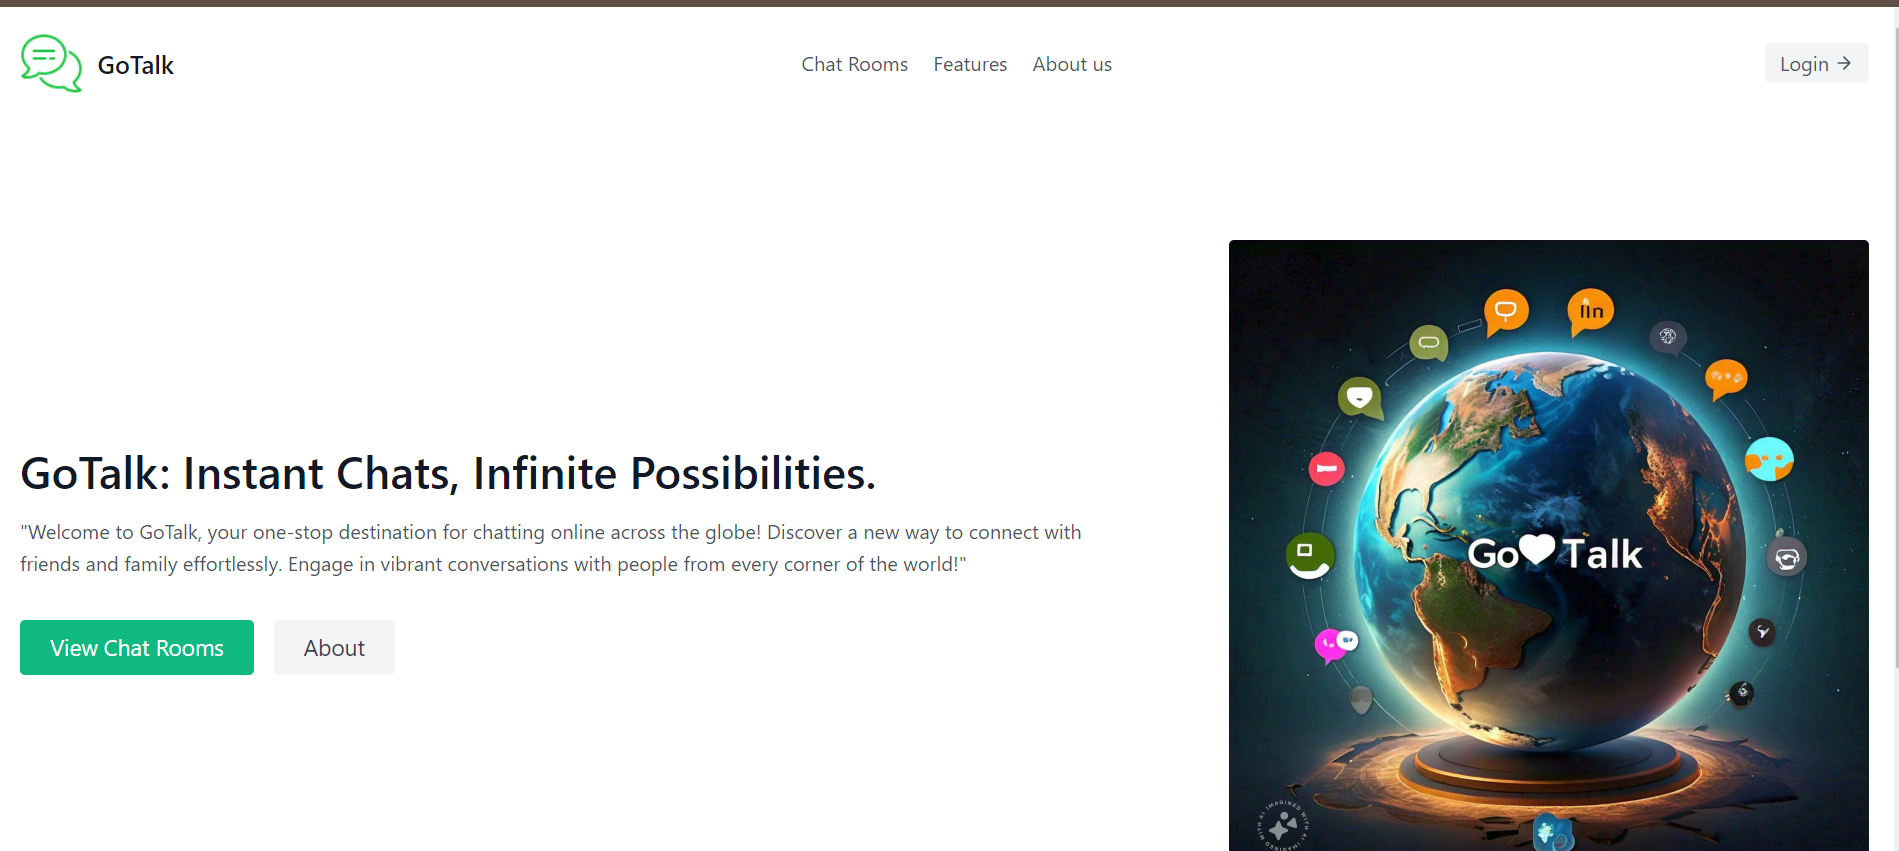
\includegraphics[width=0.9 \textwidth]{Pictures/landingpage.png}
\end{frame}

\begin{frame}{Login Page}
    \centering
    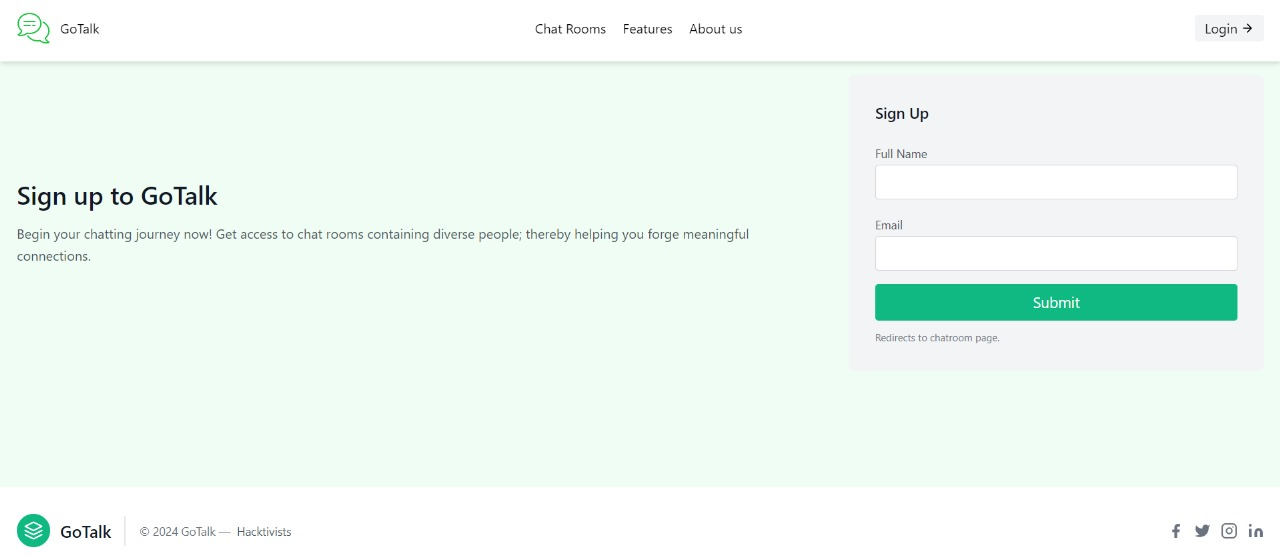
\includegraphics[width=0.9 \textwidth]{Pictures/login.jpg}
\end{frame}

\begin{frame}{Rooms Functionality}
            \centering
            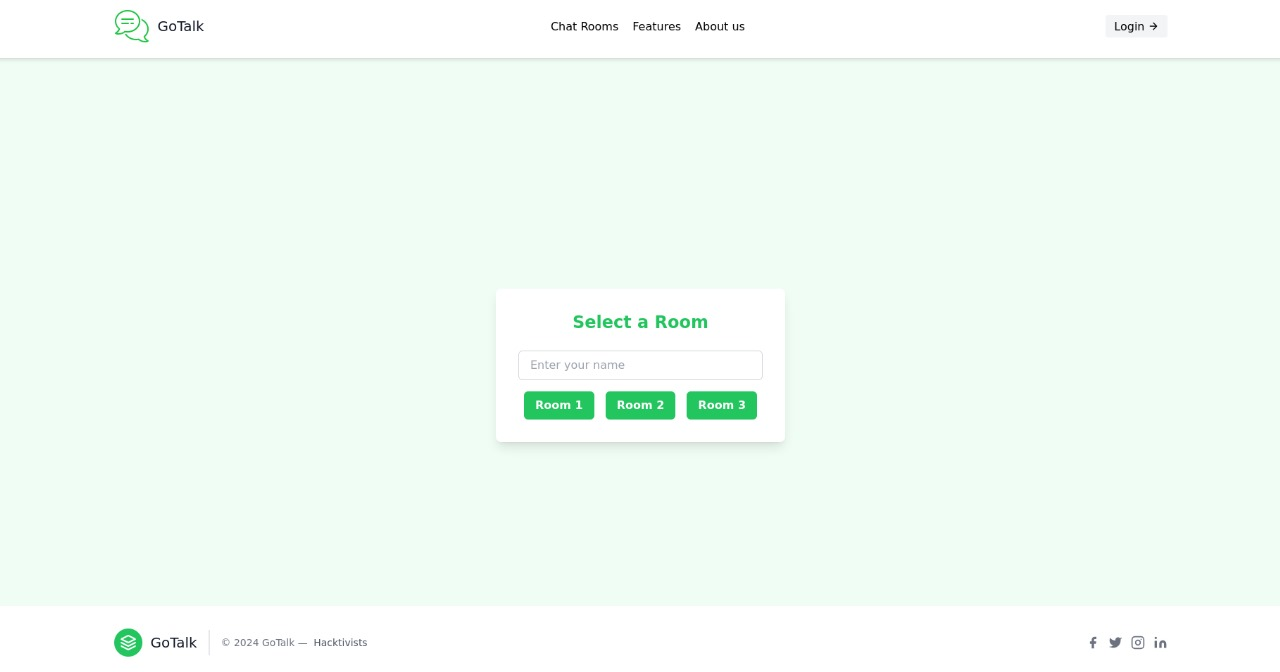
\includegraphics[width=0.9 \textwidth]{Pictures/roomselection.jpg}
\end{frame}

\begin{frame}{Chat}
    \centering
    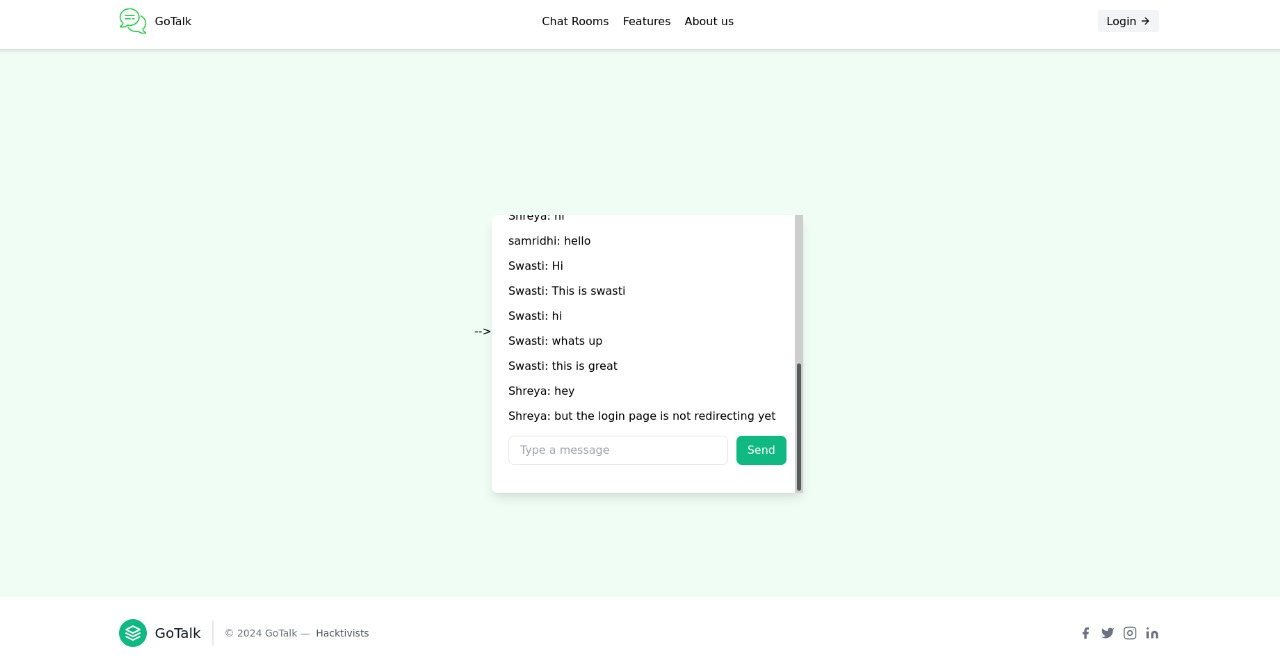
\includegraphics[width=0.9 \textwidth]{Pictures/room.jpg}
\end{frame}

\section{Conclusion}

\begin{frame}{Conclusion}
    \begin{itemize}
        \item Significant progress has been made in styling, room functionality, and cookie management. 
        \item The primary focus moving forward is resolving authentication issues and enhancing the application's overall functionality and user experience.
    \end{itemize}
    \vfill
    \begin{center}
        \textbf{Thank you for your attention!}
    \end{center}
    \begin{center}
        Suggestions and Feedback welcomed.
    \end{center}
\end{frame}

\end{document}
